\chapter{Introdução}
\epigraph{``\textit{Any fool can write code that a computer can understand. Good programmers write code that humans can understand}''.}{Martin Fowler}

\lettrine[lines=4, lhang=0.1, lraise=0, loversize=0.2, findent=0.1em]{\textcolor{niceblue}{P}}{rezado} aluno, seja bem-vindo! Este livro contém diversos Capítulos, organizados de forma a guiá-lo no processo de fixação do conteúdo aprendido em aula por meio de exercícios e projetos práticos aplicados em linguagens de programação.

Texto da revisão da literatura, dividido em seções e subseções.


Este é um exemplo de como usar figuras. Referência cruzada: Figura~\ref{fig:exemplo}

\FloatBarrier
\begin{figure}[!htbp]
    \centering
    \caption{Exemplo de figura}
    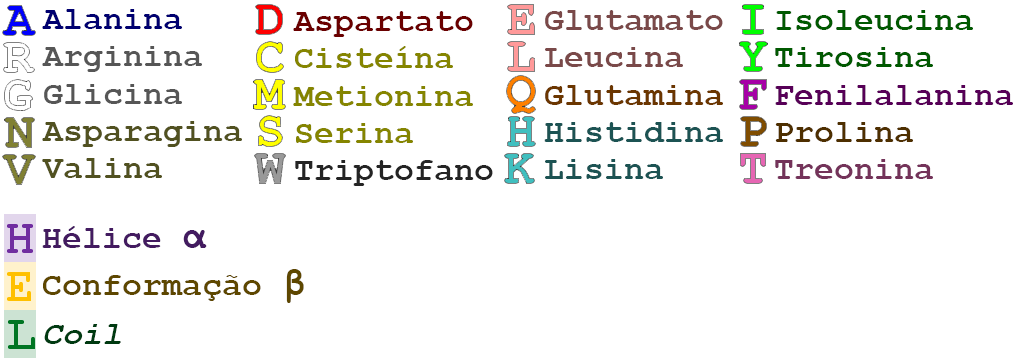
\includegraphics[scale=1.5]{imagens/teste}
    \\\textbf{Fonte:} Elaborada pelo autor
    \label{fig:exemplo}
\end{figure}
\FloatBarrier

Este é um exemplo de como usar tabelas. Referência cruzada: Tabela~\ref{tab:exemplo}

\FloatBarrier
\begin{table}[!htbp]
    \centering
    \caption{Exemplo de tabela de 2 colunas}
    \begin{tabular}{ c | c }
        \hline
        \textbf{Coluna 1} & \textbf{Coluna 2} \\ \hline
        Dado 1a           & Dado 2a           \\ \hline
        Dado 1b           & Dado 2b           \\ \hline
        Dado 1c           & Dado 2c           \\ \hline
        Dado 1d           & Dado 2d           \\ \hline
    \end{tabular}
    \\ \vspace{0.2cm}
    \textbf{Fonte:} Elaborada pelo autor
    \label{tab:exemplo}
\end{table}
\FloatBarrier


Este é um exemplo de como usar equações. Referência cruzada: Equação~\ref{eq:exemplo}

\begin{equation}
\sum_{i=1}^{n} i = \frac{n(n+1)}{2}
\label{eq:exemplo}
\end{equation}


\begin{inlineJavaCode}
public class Teste {
    public static void main( String[] args ) {
        System.out.println("teste");
    }
}
\end{inlineJavaCode}

\begin{inlineCCode}
#include <stlib.h>

int main() {
    printf("xxx");
    return 0;
}
\end{inlineCCode}

\begin{inlineCPPCode}
#include <iostream>
using namespace std;

int main() {
    cout << "cpp";
    return 0;
}
\end{inlineCPPCode}

\begin{inlineHTMLCode}
<html>
    <head></head>
    <body></body>
</html>
\end{inlineHTMLCode}

\begin{inlineJavascriptCode}
var teste = () => {
    return 1 + 2;
};

let x = 2;
\end{inlineJavascriptCode}

\javaCode{Teste.java}{fontes/Teste.java}
\cCode{Teste.c}{fontes/Teste.c}
\cppCode{Teste.cpp}{fontes/Teste.cpp}
\htmlCode{Teste.html}{fontes/Teste.html}
\javascriptCode{Teste.js}{fontes/Teste.js}


Este é um exemplo de como inserir texto sem formatação (ambiente verbatim):

\begin{verbatim}
Texto sem formatação, como espaçamento igual.
\end{verbatim}


Exemplo de lista de itens:

\begin{itemize}
    \item \textbf{Item 1:} texto...;
    \item \textbf{Item 2:} texto...;
    \begin{itemize}
        \item \textbf{Subitem:} texto...;
        \item \textbf{Subitem:} texto...;
        \item \textbf{Subitem:} texto...;
    \end{itemize}
    \item \textbf{Item 3:} texto...;
    \item \textbf{Item n:} texto....
\end{itemize}


Exemplo de lista numerada:

\begin{enumerate}
    \item \textbf{Item:} texto...;
    \item \textbf{Item:} texto...;
    \begin{enumerate}
        \item \textbf{Subitem:} texto...;
        \item \textbf{Subitem:} texto...;
        \item \textbf{Subitem:} texto...;
    \end{enumerate}
    \item \textbf{Item:} texto...;
    \item \textbf{Item:} texto....
\end{enumerate}


Exemplos de comandos para texto e referências:

\begin{itemize}
    \item Para iniciar um novo parágrafo, basta deixar uma linha em branco no código fonte;
    \item Não force o compilador a pular mais de uma linha, pois terá influência negativa na composição do documento;
    \item Sempre deixe o \LaTeX\ realizar a formatação de parágrafos e posicionamento de elementos;
    \item Utilização de aspas simples (abertura \verb|`|, fechamento \verb|'|): `Texto entre aspas simples';
    \item Utilização de aspas duplas (abertura \verb|``|, fechamento \verb|''|): ``Texto entre aspas duplas'';
    \item Negrito (comando \verb|\textbf|): \textbf{texto em negrito};
    \item Itálico (comando \verb|\textit|): \textit{texto em itálico};
    \item Sublinhado (comando \verb|\underline|): \underline{texto sublinhado};
    \item Negrito e itálico (usar comandos juntos): \textbf{\textit{texto em negrito e itálico}};
    \item Alterar cor do texto (comando \verb|\textcolor{cor}{texto}|):
    \begin{itemize}
        \item Exemplo \verb|\textcolor{red}{texto}|: \textcolor{red}{texto vermelho};
        \item Exemplo \verb|\textcolor[RGB]{255, 102, 0}|: \textcolor[RGB]{255, 102, 0}{texto laranja};
        \item Exemplo \verb|\textcolor[HTML]{006AD7}|: \textcolor[HTML]{006AD7}{texto azul};
    \end{itemize}
    \item Ambiente matemático inline (comando \verb|$ expressão $|): $s = x^2-2x +1$;
    \item Referência normal (comando \verb|\cite|):
    \begin{itemize}
        \item \cite{Agaisse1995};
        \item \cite{Abedi2014};
        \item \cite{BtNomenclature2016};
    \end{itemize}
    \item Referência normal com mais de uma obra (comando \verb|\cite|):
    \begin{itemize}
        \item \cite{Agaisse1995, Abedi2014};
        \item \cite{Nelson2014, BtNomenclature2016, AgapitoTenfen2014};
    \end{itemize}
    \item Referência nome e ano (comando \verb|\citeauthorandyear|):
    \begin{itemize}
        \item \citeauthorandyear{Agaisse1995};
        \item \citeauthorandyear{Abedi2014};
        \item \citeauthorandyear{BtNomenclature2016};
    \end{itemize}
\end{itemize}


Exemplo de nota de rodapé\footnote{Essa é uma nota de rodapé!}.

\section{teste}
\subsection{teste}
\subsubsection{teste}

